\chapter{Theoretische Grundlagen}
        \label{sec:theoretische_grundlagen}
        \section{Nichtkatalytische Partialoxidation von Erdgas}
            Die nichtkatalytische Partialoxidation (POx) von Erdgas ist ein thermochemisches Verfahren zur Herstellung von Synthesegas (Syngas), bestehend aus Kohlenstoffmonoxid (CO) und Wasserstoff (H\textsubscript{2}). Dabei reagiert Methan mit Sauerstoff, allerdings ist nicht genug Sauerstoff für eine vollständige Oxidation (Verbrennung) vorhanden. Hauptkomponente des Erdgases und Ausgangsstoff ist Methan (CH\textsubscript{4}) \cite{en16062916}.
            \begin{align}
                \mathrm{CH_4 + \frac{1}{2}\,O_2 \longrightarrow CO +2\ H_2} \qquad \Delta H_{298} = -36 \;\mathrm{kJ/mol}
            \end{align}
            Ein Teil des Methans oxidiert jedoch vollständig (Verbrennung), was zu einer stark exothermen Reaktion führt:
            \begin{align}
                \mathrm{CH_4 + 2\,O_2 \longrightarrow CO_2 + 2\,H_2O} \qquad \Delta H_{298} = -891 \;\mathrm{kJ/mol} \label{eq:vollst_oxidation}
            \end{align}
            Ein zentraler Prozessparameter ist das stöchiometrische Methan-Sauerstoff-Verhältnis, das als 
            \begin{align}
                \lambda = \frac{\mathrm{(O_2/CH_4)_{real}}}{\mathrm{(O_2/CH_4)_{stoech}}} 
            \end{align}
            definiert ist. Für eine partielle Oxidation gilt $\lambda < 1$, da Sauerstoff unterstöchiometrisch hinzugeführt wird. Dieses Verhältnis bestimmt maßgeblich die Zusammensetzung des Synthesegases sowie die Flammentemperatur. Typische Werte liegen im Bereich von 0,55 bis 0,65 \cite{Albrecht2004}.
            
            Im Vergleich zur Dampfreformierung wird durch die exotherme Oxidationsreaktion keine externe Energiezufuhr benötigt, weshalb diese Reaktion als ökonomischer betrachtet werden kann \parencite[S. 6]{en16062916}.
            Diese Reaktionen finden bei Temperaturen von über 1000~$^\circ$C statt. Da die Oxidation ohne Katalysator direkt durch Sauerstoffzufuhr erfolgt, wird eine robuste Prozessführung ermöglicht. Allerdings können dadurch auch Nebenprodukte wie Kohlenstoffdioxid (CO\textsubscript{2}), Wasserdampf und Ruß entstehen.\\
            Nach der direkten Oxidation finden in der Nachbrennzone weitere, deutlich langsamer verlaufende chemische Reaktionen statt:
            \begin{align}
                &\mathrm{CH_4 + H_2O \rightleftharpoons CO + 3\,H_2} \qquad \Delta H_{1000} = 226 \;\mathrm{kJ/mol} \label{eq:dampfreformierung}\\
                &\mathrm{CO + H_2O \rightleftharpoons CO_2 + H_2} \qquad \Delta H_{1000} = -34,5 \;\mathrm{kJ/mol}\label{eq:wassergas_shift}
            \end{align}
            Dabei ist Gleichung \ref{eq:dampfreformierung} die endotherme Dampfreformierungsreaktion, welche das nicht direkt in der Oxidation verbrauchte Methan verbraucht. Die vollständige Oxidation des Erdgases (Gleichung \ref{eq:vollst_oxidation}) liefert dabei die nötige Energie für die Dampfreformierung \cite{POX_Erdgas}.\\ 
            Falls CO\textsubscript{2} vorliegt, ist auch statt einer Reaktion mit Wasser eine Reaktion mit diesem möglich:
            \begin{align}
                &\mathrm{CH_4 + CO_2 \rightleftharpoons 2\,CO + 2\,H_2} \qquad \Delta H_{298} = 247,3 \;\mathrm{kJ/mol} \label{eq:dampfreformierung}
            \end{align}
            Da diese Reaktion kein Wasser beinhaltet, wird sie auch als "Dry Reforming"\;bezeichnet. Dieser Prozess kann zukünftig Bedeutung erlangen, um Kohlenstoffdioxid in Syngas umzuwandeln, und somit den  Ausstoß von CO\textsubscript{2} zu reduzieren \cite{LESACHE2022100970}. 
        \section{Reaktionskinetische Grundlagen}
            Die Modellierung der partiellen Oxidation (POx) von Erdgas erfordert ein tiefes Verständnis der Reaktionskinetik, da die bei dieser Partialoxidation ablaufenden Prozesse durch eine Vielzahl von Elementarreaktionen bestimmt werden. Die Reaktionskinetik beschreibt die zeitliche Änderung der Stoffmengen bzw. Konzentrationen chemischer Spezies in Abhängigkeit von Temperatur, Druck und Zusammensetzung des Reaktionsgemisches. 
            \subsection{Elementarreaktionen und Reaktionsraten}
                Die Grundlage kinetischer Modelle bildet die Annahme, dass sich komplexe Reaktionen durch die Überlagerung von Elementarreaktionen beschreiben lassen. Für jede Elementarreaktion gilt folgender Potenzansatz:
                \begin{align}
                    r_j = k_j(T)\cdot \prod_i c_i^{\nu_{ij}} \label{eq:reaktionsrate}
                \end{align}
                Dabei entspricht $r_j$ der $j$-ten Reaktion, $c_i$ der Konzentration der reagierenden Stoffe und den stöchiometrischen Koeffizienten $\nu_{ij}$. Die Geschwindigkeitskonstante $k_j$ wird dabei in der Regel durch den Arrhenius-Ansatz beschrieben:
                \begin{align}
                    k_j(T) = A_jT^{\beta}\exp\left( -\frac{E_{A,j}}{RT} \right) \label{eq:Arrhenius}
                \end{align}
                wobei $A_j$ der präexponentielle Faktor und $E_{A,j}$ die Aktivierungsenergie sind. In der vereinfachten Arrheniusgleichung gilt $\beta = 0$, allerdings zeigt sich in der Praxis, dass die Kinetik dadurch eine Abweichung erfährt. Aus diesem Grund findet man in vielen empirischen Mechanismen den Korrekturfaktor $T^\beta$ \cite{GuttelTurek2021}. 
        \subsection{Stoffbilanzen und kinetische Differentialgleichungen}
            Die zeitliche Entwicklung der Konzentration aller Spezies folgt aus der Bilanzierung der Reaktionsraten:
            \begin{align}
                \label{eq:stoffbilanz}
                \frac{dc_i}{dt}=\sum_j  \nu_{ij}r_j
            \end{align}
            Diese Gleichung stellt dabei die Quelle oder Senke eines Stoffes dar. Sie beschreibt also, wie sich die Konzentrationen jeder Spezies durch die Summe aller Reaktionsraten verändert. Dadurch stellt die Gleichung eine direkte Verbindung zwischen der Kinetik und der Stoffbilanz dar. 

            Aus Gleichungen \ref{eq:reaktionsrate} und \ref{eq:Arrhenius} geht hervor, dass die Reaktionsrate von der Temperatur abhängig ist. Dies führt zu einem System nichtlinearer Differentialgleichungen (ODEs), dessen Lösung die Kinetik des betrachteten Reaktionssystems beschreibt. Für Prozesse wie die Partialoxidation müssen dabei mehrere hundert bis tausend Elementarreaktionen berücksichtigt werden (siehe Tabelle  \ref{tab:reaktionsmechanismen_überblick}) \cite{GuttelTurek2021}.
    \section{Thermodynamische Grundlagen}
        Neben der Reaktionskinetik bilden die thermodynamischen Rahmenbedingungen die zweite wesentliche Grundlage zur Modellierung der partiellen Oxidation. Sie bestimmen die Gleichgewichtslagen, die Energiebilanz sowie die Temperaturentwicklung im Reaktor, und haben somit direkten Einfluss auf die  Reaktionskinetik (siehe Gleichung \ref{eq:Arrhenius}).
        \subsection{Chemisches Gleichgewicht und freie Enthalpie}
            Die treibende Kraft für chemische Reaktionen ist die Änderung der Gibbs-Energie $G$. Für eine Reaktion mit den stöchiometrischen Koeffizienten $\nu_i$ gilt:
            \begin{align}
                \Delta_rG(T,p) = \sum_i\nu_i\mu_i(T,p)
            \end{align}
            mit den chemischen Potentialen $\mu_i$. Da sich im Gleichgewicht die Konzentrationen nicht mehr ändern, gilt:
            \begin{align}
                \Delta_rG=0
            \end{align}
            Die Lage des Gleichgewichts kann über die Gleichgewichtskonstante $K$ ausgedrückt werden, 
            \begin{align}
                &\Delta_rG^\circ(T) = -RT \ln K  \\
                & K(T) = \exp \left( - \frac{\Delta_rG^\circ(T)}{RT}\right)
            \end{align}
            die mit der Standardreaktionsenthalpie $\Delta_rH^\circ$ und der Standardreaktionsentropie $\Delta_rS^\circ$ über Gleichung \ref{eq:gibbs_helmholtz} (Gibbs-Helmholtz-Gleichung) verknüpft ist.
            \begin{align}
                \Delta_r G^\circ(T) &= \Delta_r H^\circ(T) - T \, \Delta_r S^\circ(T) \label{eq:gibbs_helmholtz}
            \end{align}
            Für die POx ist relevant, dass sowohl exotherme (z.B. Reaktion  \ref{eq:vollst_oxidation}) als auch endotherme (vgl. siehe Reaktion \ref{eq:dampfreformierung}) Reaktionen auftreten, wodurch konkurrierende Gleichgewichte entstehen. 
        \subsection{Energiebilanz der Reaktion}
            Die Temperaturentwicklung im Reaktor wird über die Energiebilanz beschrieben:
            \begin{align}
                \rho c_p \frac{dT}{dt} = -\sum_j\Delta_rH_jr_j + Q_{Verlust}
            \end{align}
            Der erste Term berücksichtigt dabei die durch die Reaktion entstehende oder aufgenommene Reaktionsenthalpie. Der zweite Term beschreibt Wärmeverluste des Reaktors. Für die Partialoxidation typisch ist eine Kombination aus exothermen (Oxidation von Methan) und endothermen Reaktionen (Dampfreformierung). Dadurch kommt es im Reaktor sowohl zu Temperaturspitzen (Flammzone), als auch zu Bereichen mit deutlich geringerer Temperatur (Reformierungsbereich). 
        \subsection{Relevanz für die Simulation}
            Die thermodynamischen Daten sind notwendig, um die Energiebilanz im Reaktor korrekt zu berechnen, die Temperaturabhängigkeit der Reaktionsgeschwindigkeiten korrekt abzubilden und die Gleichgewichtszusammensetzungen zu bestimmen.

            Chemkin nutzt dazu Reaktionsmechanismen, die sowohl reaktionskinetische als auch thermodynamische Daten enthalten. Nur durch die simultane Lösung von Stoff- und Energiebilanzen kann das Reaktorverhalten realistisch abgebildet werden.
    \section{Reduced-Order Models (ROMs)}
        Die detaillierte Simulation chemischer Reaktoren auf Basis vollständiger Strömungs- und Reaktionssimulationen mit Computational Fluid Dynamics (CFD) ist mit einem sehr hohen Rechenaufwand verbunden. Besonders bei der partiellen Oxidation von Erdgas, bei der hunderte Reaktionen berücksichtigt werden müssen, stellt eine komplexe Simulation mit CFD-Modellen eine große Herausforderung dar. Reduced-Order Models (ROMs) stellen eine Methode dar, diese Komplexität zu verringern, indem nur wesentliche physikalisch-chemische Prozesse explizit beschrieben werden.
        
        %Die Grundidee von ROMs ist es, Modelle zu entwickeln, welche die wesentlichen Größen, darunter Temperatur- und Konzentrationsprofile sowie Umsatz, mit deutlich verringertem Rechenaufwand vorherzusagen. Damit eignen sie sich sowohl für Prozesssimulation als auch für komplexe Optimierungsaufgaben und Parameterstudien, bei denen zahlreiche Modellberechnungen notwendig sind. Darüber hinaus ermöglichen ROMs Anwendungen in der Echtzeit-Prozessführung, der Regelungstechnik und der Prozessoptimierung, bei denen detaillierte CFD-Modelle zu langsam wären. Allerdings bleibt die Modellgüte auf die Genauigkeit der zugrunde liegenden Reduktion und Annahmen beschränkt.

        ROMs kombinieren dabei null- und eindimensionale, idealisierte Reaktoren, um ein umfangreiches Modellnetzwerk zu beschreiben. Sie ermöglichen es, mit einem geringen Rechenaufwand wesentliche Informationen über das Prozessverhalten zu erhalten. Dadurch eignen sich diese Modelle für umfangreiche Parameterstudien oder Optimierungsalgorithmen, die eine hohe Anzahl an Simulationen in einer kurzen Zeit ausführen. Darüber hinaus ermöglichen ROMs Anwendungen in der Echtzeitprozessführung, der Regelungstechnik und der Prozessoptimierung, bei denen detaillierte CFD-Modelle zu langsam wären. Allerdings bleibt die Modellgüte auf die Genauigkeit der zugrunde liegenden Reduktion und Annahmen beschränkt.

        Trotz dieser Vorteile gibt es bislang wenige Arbeiten, die sich mit der Entwicklung, Validierung und Anwendung für ROMs für reaktive Systeme beschäftigen. Viele der veröffentlichten Modelle dienen vielmehr der Validierung von Teilmodellen für CFD-Berech\-nungen oder neuer Reaktionsmechanismen und sind daher nicht in der Lage, die fundamentalen Phänomene abzubilden \cite{VOLOSHCHUK2022117620}.
    \section{Reaktortypen}
        %Ein zentrales Konzept bei der Nutzung von reduced order models ist die Nutzung idealisierter Reaktortypen, wie dem Perfectly Stirred Reactor (PSR) und dem Plug Flow Reactor (PFR). Diese beiden Modelle dienen als Bausteine für komplexere Reaktornetzwerke.

        Ein zentrales Konzept bei der Entwicklung und Anwendung von Reduced-Order-Models (ROMs) ist die Nutzung idealisierter Reaktorkonzepte. Diese Modelle abstrahieren die physikalischen Vorgänge auf wenige charakteristische Größen, um wesentliche Transport- und Reaktionsphänomene mit geringem Rechenaufwand abzubilden. Zwei der am häufigsten verwendeten Reaktormodelle sind der Perfectly Stirred Reactor (PSR) und der Plug Flow Reactor (PFR). Beide Modelle dienen als fundamentale Bausteine für komplexe Reaktornetzwerke, mit denen reale Prozesse näherungsweise beschrieben werden können.
        
        \subsection{Perfectly Stirred Reactor (PSR)}
            %Der PSR beschreibt ein vollständig durchmischtes Reaktionsvolumen ohne Temperatur- und Konzentrationsgradienten. Für ROMs bietet er mehrere Anwendungsmöglichkeiten, darunter die Abbildung stark turbulenter und durchmischter Teilbereiche wie die Flammzone. Dabei ist der Vorteil, dass einfache Bilanzgleichungen eine schnelle Berechnung erlauben.

            Der Perfectly Stirred Reactor beschreibt ein ideal durchmischtes Reaktionsvolumen, in dem Temperatur, Dichte und Stoffmengenanteile im gesamten Reaktor homogen sind. Es existieren somit keine räumlichen Gradienten. Diese Annahme erlaubt eine starke Vereinfachung der Bilanzgleichungen, da nur zeitliche Änderungen der Zustandsgrößen betrachtet werden müssen. Unter stationären Bedingungen entspricht der PSR einem kontinuierlich betriebenen Rührkessel (Continuous Stirred Tank Reactor, CSTR). 

            Die allgemeine Stoffbilanz für eine Komponente $i$ im PSR lautet \cite{Emig_Klemm_2017}:
            \begin{align}
                \frac{\mathrm{d}n_i}{\mathrm{d}t} &= \dot n_{i,0} - \dot n_i + V \cdot \sum_{j=1}^M \nu_{i,j}r_j\\
                &=\dot V\cdot c_{i,0} - \dot V\cdot c_i + V \cdot \sum_{j=1}^M \nu_{i,j}r_j \label{eq:stoffbilanz_psr}
            \end{align}
            Gleichung \ref{eq:stoffbilanz_psr} gilt dabei unter der Annahme, dass eine konstante Dichte vorherrscht. 
            Hierbei bezeichnet $\frac{\mathrm{d}n_i}{\mathrm{d}t}$ die Änderung der Stoffmenge (bzw. Konzentration), $c_{i,0}$ die Eingangskonzentration, $c_i$ die Konzentration des Stoffes i und $\dot V$ den Volumenstrom. Der hintere Term beschreibt die Quellen/Senken des Stoffes durch die chemischen Reaktionen. 
            
            Im Falle eines stationär betriebenen Reaktors gilt:
            \begin{align}
                \frac{\mathrm{d}n_i}{\mathrm{d}t} = 0
            \end{align}

            Analog lässt sich mit Gleichung \ref{eq:enthalpiebilanz_psr_1} bzw. \ref{eq:enthalpiebilanz_psr_2} die Enthalpiebilanz beschreiben,
            \begin{align}
                \frac{dU}{dt}&=\dot Q_{ein} - \dot Q_{aus} + \dot{Q}_{Verl} + \dot Q_{Quelle} \label{eq:enthalpiebilanz_psr_1}
                \\
                \frac{d\left(V \cdot \rho c_p T\right)}{dt} 
                &= \dot{V}_0 \rho_0 c_{p,0} T_0 
                - \dot{V} \rho c_p T 
                + k_w A_W (\overline{T}_{WT} - T) 
                + V \cdot \sum_{j=1}^{M} \left( r_j \cdot (-\Delta_R H_j) \right) \label{eq:enthalpiebilanz_psr_2}
            \end{align}
            wobei für den stationären Fall entsprechend gilt: 
            \begin{align}
                \frac{d\left(V \cdot \rho c_p T\right)}{dt}  = 0.
            \end{align}

            $\dot Q_{ein}$ und $\dot Q_{aus}$ beschreiben dabei die durch den Massenstrom zu- bzw. abgeführte Enthalpieströme, und $\dot Q_{Quelle}$ die Enthalpie aus einer exo- bzw. endothermen Reaktion \cite{Emig_Klemm_2017}. $\dot Q_{Verl}$ ist durch den konvektiven Wärmeübergang 
            \begin{align}
                \dot Q_{Verl} = k_w A_W (\overline{T}_{WT} - T) 
            \end{align}
            beschrieben. Dabei ist $k_w$ der Wärmeübergangskoeffizient, $A_W$ die Wandfläche und $\overline{T}_{WT} - T$ die Temperaturdifferenz zwischen dem Medium und der Umgebung.
            
            Da keine Gradienten auftreten, ist das System durch einen Satz gewöhnlicher Differentialgleichungen (ODEs) vollständig beschrieben. Dies macht einen PSR zu einem effizienten Werkzeug in kinetischen Studien mit einem sehr geringen Rechenaufwand.
            
        \subsection{Plug Flow Reactor (PFR)}
            %Der PFR modelliert eine strömende Reaktionszone mit axialen Gradienten, jedoch ohne radiale Durchmischung. Er eignet sich, um axiale Temperatur- und Konzentrationsprofile in Rohrreaktoren oder nachgeschalteten Reformierungszonen zu betrachten.

            Im Gegensatz dazu beschreibt der Plug Flow Reactor (PFR) eine strömende Reaktionszone, in der das Fluid als Folge infinitesimal dünner Strömungselemente ohne radiale Durchmischung durch den Reaktor transportiert wird. Innerhalb eines jeden Strömungselements wird dabei vollständige Vermischung angenommen. Entlang der axialen Richtung entstehen so Temperatur- und Konzentrationsgradienten. 

            Die allgemeine Stoffbilanz eines PFRs lautet,
            \begin{align}
                \frac{\partial c_i}{\partial t} = -u_z \frac{\partial c_i}{\partial z} + \sum_{j=1}^M \nu_{ij}r_j
            \end{align}
            wobei $u_z$ die Strömungsgeschwindigkeit entlang der axialen Koordinate ist.

            Die Enthalpiebilanz lautet entsprechend:
            \begin{align}
                \rho c_p \frac{\partial T}{\partial t} = -\rho c_p u_z \frac{\partial T}{\partial z} + \sum_{j=1}^M (r_j\cdot (-\Delta_RH_j)) + \dot q_{Verl}
            \end{align}
            $\dot q_{Verl}$ ist dabei die Wärmestromdichte. 

            Wie beim PSR gilt auch bei dem PFR für den stationären Fall: 
            \begin{align}
                \frac{\partial T}{\partial t} = \frac{\partial c_i}{\partial t} = 0
            \end{align}
            
            Im Gegensatz zum PSR ist der PFR damit ein eindimensionales Modell, das über gekoppelte Differentialgleichungen (gewöhnliche oder partielle) gelöst wird. Es eignet sich sehr gut zur Beschreibung von Rohrreaktoren oder nachgeschalteten Reformierungszonen, in denen die Durchmischung in Strömungsrichtung gering ist \cite{Emig_Klemm_2017}. 
    \section{Literaturrecherche}
        \subsection{Wahl des Reaktionsmechanismus}
            \label{sec:reaktionsmechanismen_literatur}
            Für die Modellierung der POx ist die Auswahl des Reaktionsmechanismus ein entscheidendes Kriterium. Verschiedene Reaktionsmechanismen führen sowohl zu anderen kinetischen Ergebnissen als auch zu deutlich verschiedenen Rechenzeiten und nume\-rischen Stabilitäten. 

            Entsprechend besteht ein hohes Interesse an der Validierung verschiedener Reaktions\-mechanismen. Ursprünglich wurde ein Großteil der für diese Anwendungen genutzten Mechanismen jedoch für direkte Verbrennungsprozesse entwickelt und validiert~\cite{MILLER2021100886}. Umfangreiche Validierungsuntersuchungen für den Prozess der partiellen Oxidation wurden kaum durchgeführt, weshalb eine Untersuchung der Mechanismen unter bestimmten Prozessbedingungen erforderlich ist. Eine direkte Übertragung der Ergebnisse aus Verbrennungsstudien auf POx-Systeme ist aufgrund der stark unterschiedlichen Prozessbedingungen nur eingeschränkt möglich.

            Paykani et al. untersuchten die Flammeneffekte methanhaltiger Brennstoffe und stellten fest, dass alle in der Studie betrachteten Mechanismen ähnliche Resultate mit nur geringen Abweichungen aufweisen. Der GRI-Mech zeigte dabei trotz seiner vergleichsweise geringen Speziesanzahl eine gute Balance zwischen Genauigkeit und Rechenaufwand \cite{en14102834}. 

            In einer Vergleichsstudie untersuchten Zhang et al. 45 Publikationen, die sich mit der Modellvalidierung für die Verbrennung von Methan unter vielfältigen Bedingungen beschäftigen. Unter den beobachteten Spezies befinden sich umfangreiche Kohlenwasserstoffe und Aromaten, teilweise auch Radikale. Als verdünnende Gase wurden unter anderem Stickstoff (N$_2$), Wasserdampf(H$_2$O) und Kohlenstoffdioxid (CO$_2$) berücksichtigt. In Abbildung \ref{fig:mechanismusvergleich_zhang} ist erkennbar, dass Aramco in vielen Bereichen den geringsten Fehler aufweist, was durch die hohe Anzahl an Vergleichsstudien eine wichtige Erkenntnis zur Wahl des Reaktionsmechanismus darstellt. 

            Zur Bewertung der Mechanismen wurden in \textcite{ZHANG2025114499} verschiedene experimentelle Datensätze herangezogen, 
            die unterschiedliche Reaktorkonzepte abbilden. Dabei bezeichnet \textbf{FR} einen \textit{(Plug)-Flow-Reactor}, in dem stationäre Gasphasenreaktionen unter definierten Temperatur- und Druckbedingungen untersucht werden. 
            \textbf{JSR} steht für \textit{Jet-Stirred Reactor}, einen gut durchmischten Rührreaktor, der eine homogene Temperaturverteilung ermöglicht 
            und häufig zur Analyse von Produktspezies am Reaktorausgang verwendet wird. 
            \textbf{ST} beschreibt ein \textit{Shock Tube}, ein Stoßrohr, das kurzzeitig homogene Hochtemperatur- und Hochdruckbedingungen erzeugt, 
            um Zündverzögerungszeiten und zeitabhängige Speziesprofile zu messen. 
            Die Indizes \textbf{out}, \textbf{t} und \textbf{spec} kennzeichnen dabei, ob sich die Validierung auf Spezieskonzentrationen am Reaktorausgang, 
            auf zeitabhängige Größen (z.\,B. Zündverzögerungszeiten) oder auf detaillierte Speziesprofile bezieht.

            \begin{figure}[H]
                \centering
                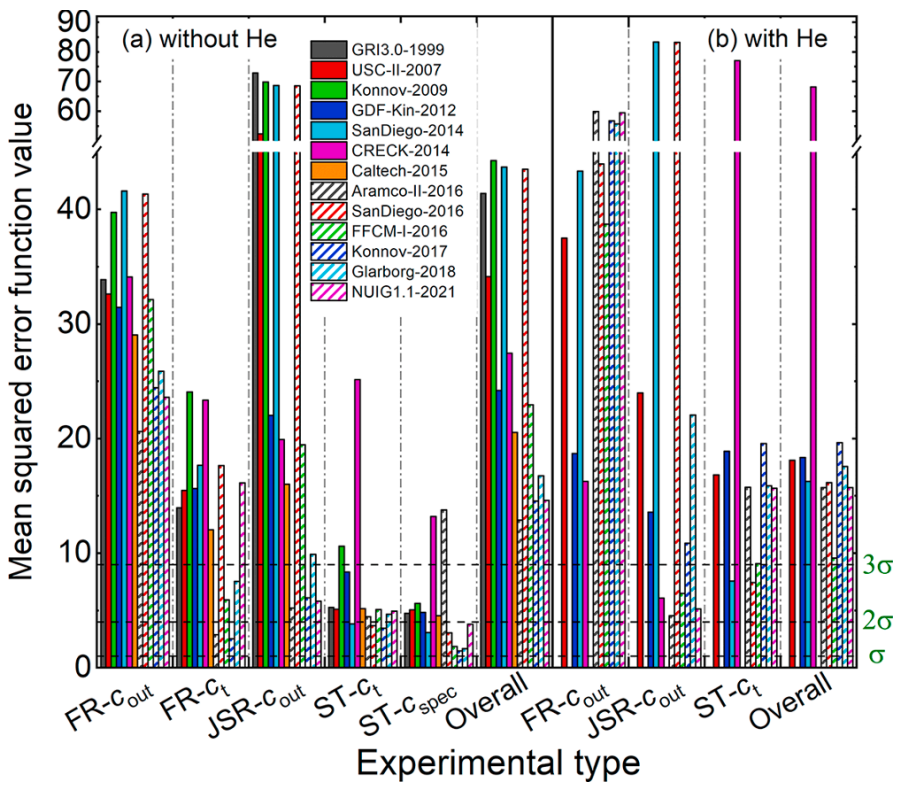
\includegraphics[width=0.65\linewidth]{img/sonstiges/Mechanismusvergleich_Zhang.png}
                \caption{Mittlerer quadrierter Fehler verschiedener Reaktionsmechanismen in Simulationen ohne (a) und mit (b) Helium aus einer Vergleichsstudie \cite{ZHANG2025114499}.}
                \label{fig:mechanismusvergleich_zhang}
            \end{figure} 
            Aufgrund der großen Menge an Daten in Abbildung \ref{fig:mechanismusvergleich_zhang} werden ausgewählte Zahlenwerte in Tabelle \ref{tab:zhang_mechanismen_auszug} dargestellt.
            \begin{table}[H]
                \centering
                \caption{Auszug aus den mittleren quadratischen Fehlerwerten (Mean Squared Error Function Values) verschiedener Mechanismen ohne Helium nach \textcite{ZHANG2025114499}.}
                \begin{tabular}{lcccccc}
                \toprule
                Mechanismus & FR$_\text{out}$ & FR$_\text{t}$ & JSR$_\text{out}$ & ST$_\text{t}$ & ST$_\text{spec}$ & Overall \\
                \midrule
                GRI3.0--1999   & 33.87 & 13.96 & 72.90 & 5.25 & 4.75 & 41.39 \\
                CRECK--2014    & 34.10 & 23.37 & 19.91 & 15.24 & 13.20 & 27.46 \\
                Aramco--II--2016 & 20.60 & 2.87 & 5.20 & 4.43 & 13.76 & 12.86 \\
                NUIG1.1--2021  & 23.59 & 16.12 & 5.79 & 4.94 & 3.81 & 14.61 \\
                \bottomrule
                \end{tabular}
                \label{tab:zhang_mechanismen_auszug}
            \end{table}
            Als Ergebnis dieser Studie wird Aramco-II-16 als zuverlässigster Reaktionsmechanismus genannt \cite{ZHANG2025114499}. 

            Zettervall et al. untersuchten die Anwendbarkeit von Reaktionsmechanismen für CFD-Analysen und fanden, dass Aramco die besten Ergebnisse liefert. Da CFD-Simulationen allerdings einen deutlich höheren Rechenbedarf erfordern, muss für die Anwendung dieses Mechanismus dieser stark reduziert werden. Insgesamt zeigt diese Studie jedoch, dass die meisten Mechanismen vergleichbare Ergebnisse liefern \cite{fuels2020013}. 

            In der Literatur finden sich nur wenige Arbeiten, die sich explizit mit der numerischen Effizienz chemischer Reaktionsmechanismen befassen. Der Einfluss der Komplexität des Mechanismus, insbesondere die Anzahl der Spezies und Elementarreaktionen, auf den Rechenaufwand wird meist nur theoretisch beschrieben \parencite{Niemeyer2016, CURTIS2017312}, eine systematische Quantifizierung anhand praktischer Simulationen ist jedoch selten, speziell im Gebiet der partiellen Oxidation. 
            Eine solche Analyse bietet hohes Potenzial, um Mechanismen nicht nur hinsichtlich ihrer berechneten Ergebnisse, sondern auch hinsichtlich ihrer Recheneffizienz zu beurteilen. 

            Zusammenfassend lässt sich feststellen, dass alle Reaktionsmechanismen ähnliche Ergebnisse liefern. Obwohl einige Studien die Verbrennungscharakteristiken von Methan untersuchen, ist eine Übertragbarkeit auf die partielle Oxidation möglich. Alle aufgeführten Mechanismen wurden zusätzlich unter den Bedingungen der hier betrachteten Versuchsanlage validiert. Insbesondere die Vergleichsstudie deutet darauf hin, dass der Reaktionsmechanismus Aramco tendenziell den geringsten Fehler aufweist. Dabei bietet Aramco zudem einen guten Kompromiss aus Genauigkeit, Detaillierungsgrad und Rechenaufwand.